\documentclass[tikz,border=2mm]{standalone}

\usetikzlibrary{arrows,positioning}

\begin{document}

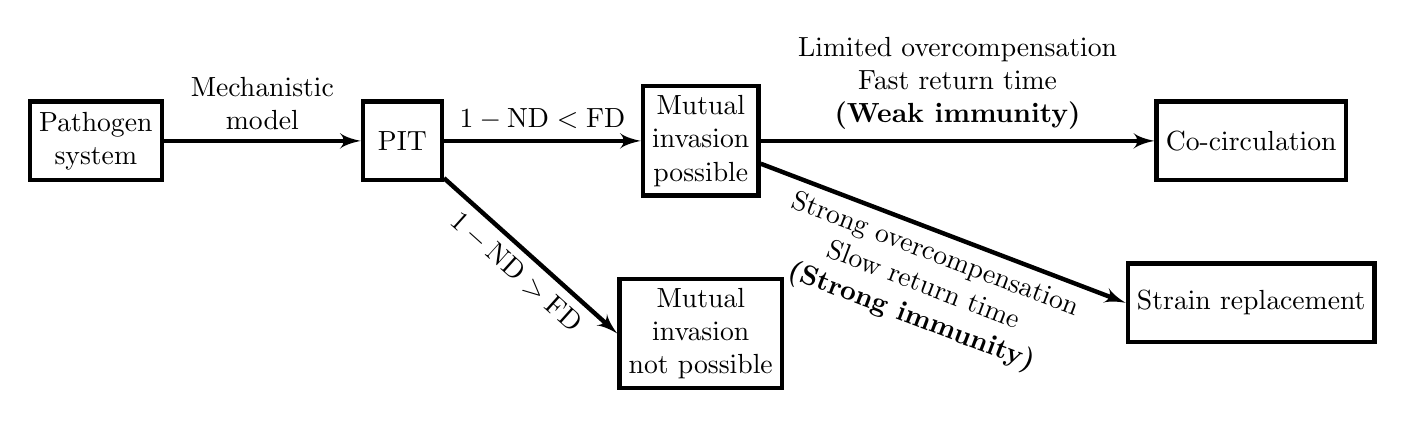
\begin{tikzpicture}[node distance=5cm,auto,>=latex',every node/.append style={align=center},int/.style={draw, minimum size=1cm},inverter/.style={rectangle,draw,inner sep=2pt,minimum size=6mm},]
    \node [int, ultra thick] (box1)             {Pathogen\\system};
    \node [int, right=2.5cm of box1, ultra thick] (box2)             {PIT};
    \node [int, right=2.5cm of box2, ultra thick] (box3)             {Mutual\\invasion\\possible};
    \node [int, below=1cm of box3, ultra thick] (box4)             {Mutual\\invasion\\not possible};
    \node [int, right=of box3, ultra thick] (box5)             {Co-circulation};
    \node [int, below=1cm of box5, ultra thick] (box6)             {Strain replacement};
    \path[->, ultra thick] (box1) edge node [above] {Mechanistic\\model} (box2);
    \path[->, ultra thick] (box2) edge node [above] {$1-\mathrm{ND}<\mathrm{FD}$} (box3);
    \path[->, ultra thick, sloped] (box2) edge node [below] {$1-\mathrm{ND}>\mathrm{FD}$} (box4.west);
    \path[->, ultra thick] (box3) edge node [above] {Limited overcompensation\\Fast return time\\\textbf{(Weak immunity)}} (box5);
    \path[->, ultra thick, sloped] (box3) edge node [below] {Strong overcompensation\\Slow return time\\\textbf{(Strong immunity)}} (box6.west);
\end{tikzpicture}
\end{document}